\documentclass{report}
\usepackage{subfig}
\usepackage{graphicx}
\usepackage{float}
\usepackage[margin=1in]{geometry}
\graphicspath{ {./images/} }
\DeclareGraphicsExtensions{.pdf}

\begin{document}

\title{\textbf{Project Watt} \\ LCOM Final Report \\ Turma 6 - Grupo 7}
\author{Eduardo da Costa Correia\\
\texttt{up201806433}
\and
Tiago Duarte Silva\\
\texttt{up201806516}}   
\maketitle

\tableofcontents

\chapter{Instruções de Utilização} 

\section{Menu Principal}

Ao iniciar o programa, é apresentada o menu principal, onde o jogador pode selecionar um dos dois modos de jogos possíveis a iniciar, cada um com a opção de se jogar ou não com outro jogador.

Para sair do jogo, o utilizador deve pressionar a tecla \textbf{\textit{Esc}} duas vezes, o mesmo para voltar ao menu principal a partir de um dos modos de jogo.

\begin{figure}[H]
	\centering
	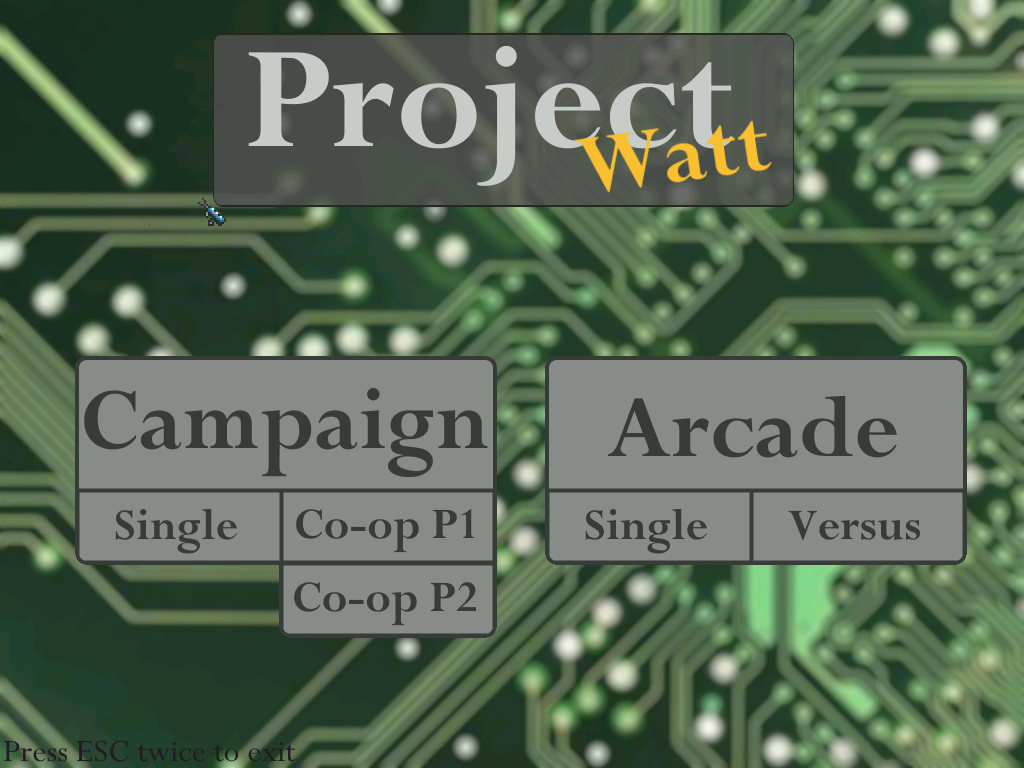
\includegraphics[width=0.9\textwidth]{main_menu}
	\caption{Menu principal}
\end{figure}

\pagebreak

\section{Campaign}

Este é o modo de jogo "principal" em que um jogador controla a personagem \textit{Watt} (Figura \ref{fig:watt}), uma faísca que ficou "presa" num curto-circuito e que para sair terá de fazer "ligação à terra" (Figura \ref{fig:exit}), ou seja, neste caso, a personagem tem de alcançar o \textbf{canto superior direito do mapa} (Figura \ref{fig:level}\footnotemark). Para isso tem de ultrapassar diversos obstáculos tais como os \textbf{espinhos} e \textbf{lasers} (se tocar num destes a faísca dissipa-se e volta ao início).

Para além disso, é possível controlar certos aspetos da jogabilidade, como a \textbf{altura do salto} da personagem e a sua \textbf{velocidade} (através dos \textit{sliders} azul e laranja respetivamente). 

Existem ainda dois \textbf{powerups} que após obtidos, desbloqueiam o controlo de funcionalidades adicionais, requeridas para acabar o nível. Estes são o powerup dos \textbf{lasers} (\textbf{canto superior esquerdo} - Figura 1.3) que permitem controlar qual dos lasers está \textbf{inativo} (vermelho, azul ou roxo - através dos botões com a cor correspondente) e alterar o sentido da gravidade da personagem (ou seja, a personagem passa a ser puxada para cima em vez de para baixo como seria normalmente). 

Todos estes aspetos são controlados pelo \textbf{segundo jogador}se estiver a jogar em co-op através de uma \textbf{\textit{switchboard}} (Figura \ref{fig:switchboard}). Esta \textbf{\textit{switchboard}} possui ainda um \textbf{\textit{mini-jogo}} que consiste em destruir \textbf{\textit{balões}} que aparecem (clicando neles) antes que estes atinjam o \textbf{topo do ecrã}, caso contrário, tal gerará \textbf{\textit{interferência}} (o ecrã fica com \textit{ruído} para tornar a experiência mais desafiante e fazer com que quem controle a personagem 2 tenha de estar mais ativo).

\begin{figure}[H]
	\centering
	
\includegraphics{watt}
	\caption{Personagem 1 - Watt}
	\label{fig:watt}
\end{figure}

\begin{figure}[H]
	\centering
	
\includegraphics[width=0.08\textwidth]{exit_icon}
	\caption{Saída}
	\label{fig:exit}
\end{figure}

\begin{figure}[H]
    \centering
    \subfloat[Laser]{{
\includegraphics{laser_icon} }}%
    \qquad
    \subfloat[Anti-gravidade]{{
\includegraphics{anti_gravity_icon} }}
    \caption{Powerups}
    \label{fig:powerups}
\end{figure}

\footnotetext{As figuras apresentadas para ilustrar o nível da personagem 1 do modo campaign são do modo singleplayer, portanto incluem botões e \textit{sliders} no canto superior esquerdo que não estão presentes no modo \textit{co-op}}

\pagebreak

\begin{figure}[H]
	\centering
	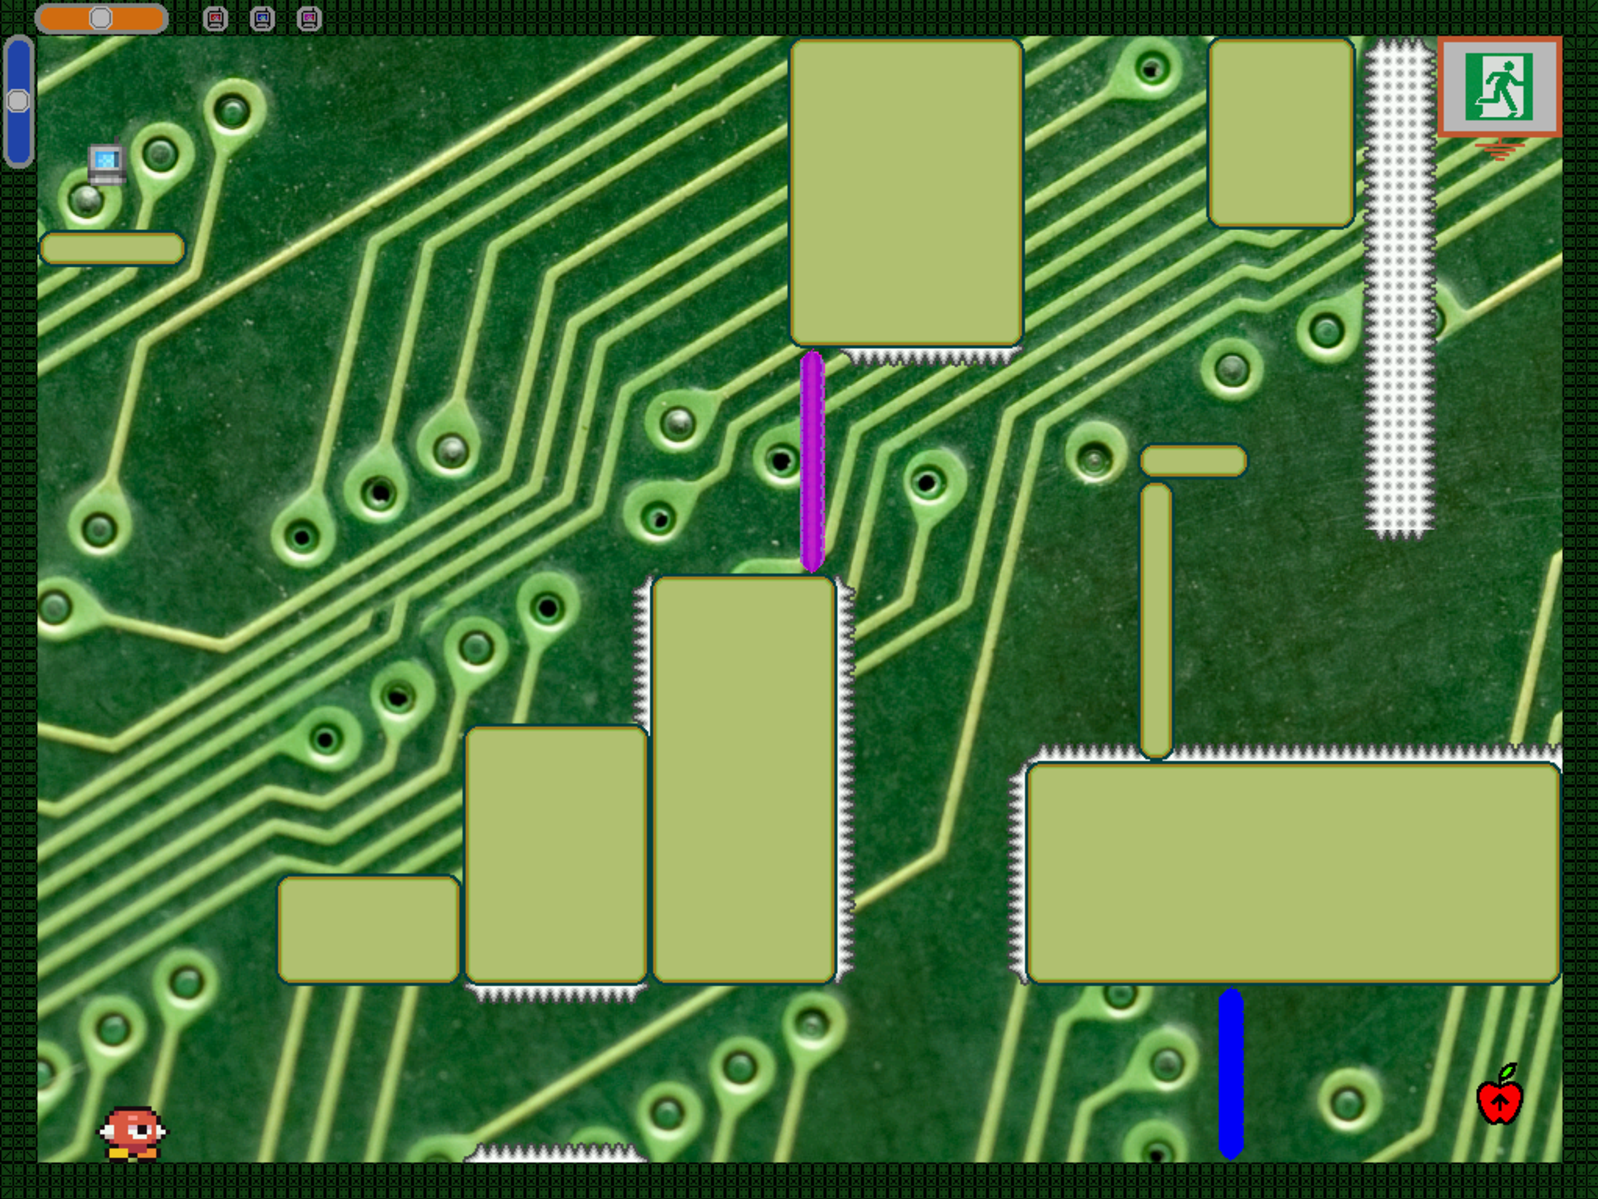
\includegraphics[width=0.8\textwidth]{campaign_singleplayer}
	\caption{Campaign - Nível (Personagem 1)}
	\label{fig:level}
\end{figure}

\begin{figure}[H]
	\centering
	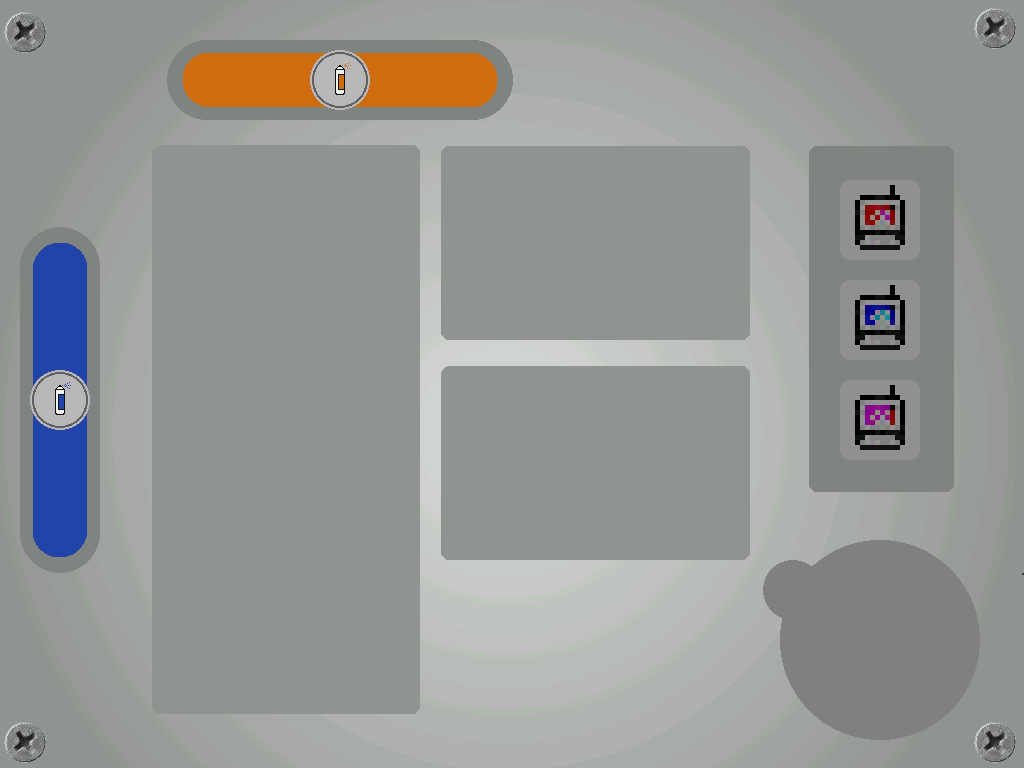
\includegraphics[width=0.8\textwidth]{campaign_switchboard}
	\caption{Campaign - Switchboard (Personagem 2)}
	\label{fig:switchboard}
\end{figure}

\pagebreak

\subsection{Victory Screen}

Quando o jogador conclui o modo \textbf{\textit{Campaign}}, é exibido um ecrã a parabenizá-lo e a informá-lo do \textbf{tempo que demorou}, em segundos, a fazê-lo.
Para sair deste ecrã e regressar ao menu principal o utilizador deve pressionar \textbf{\textit{Esc}} duas vezes.

\begin{figure}[H]
	\centering
	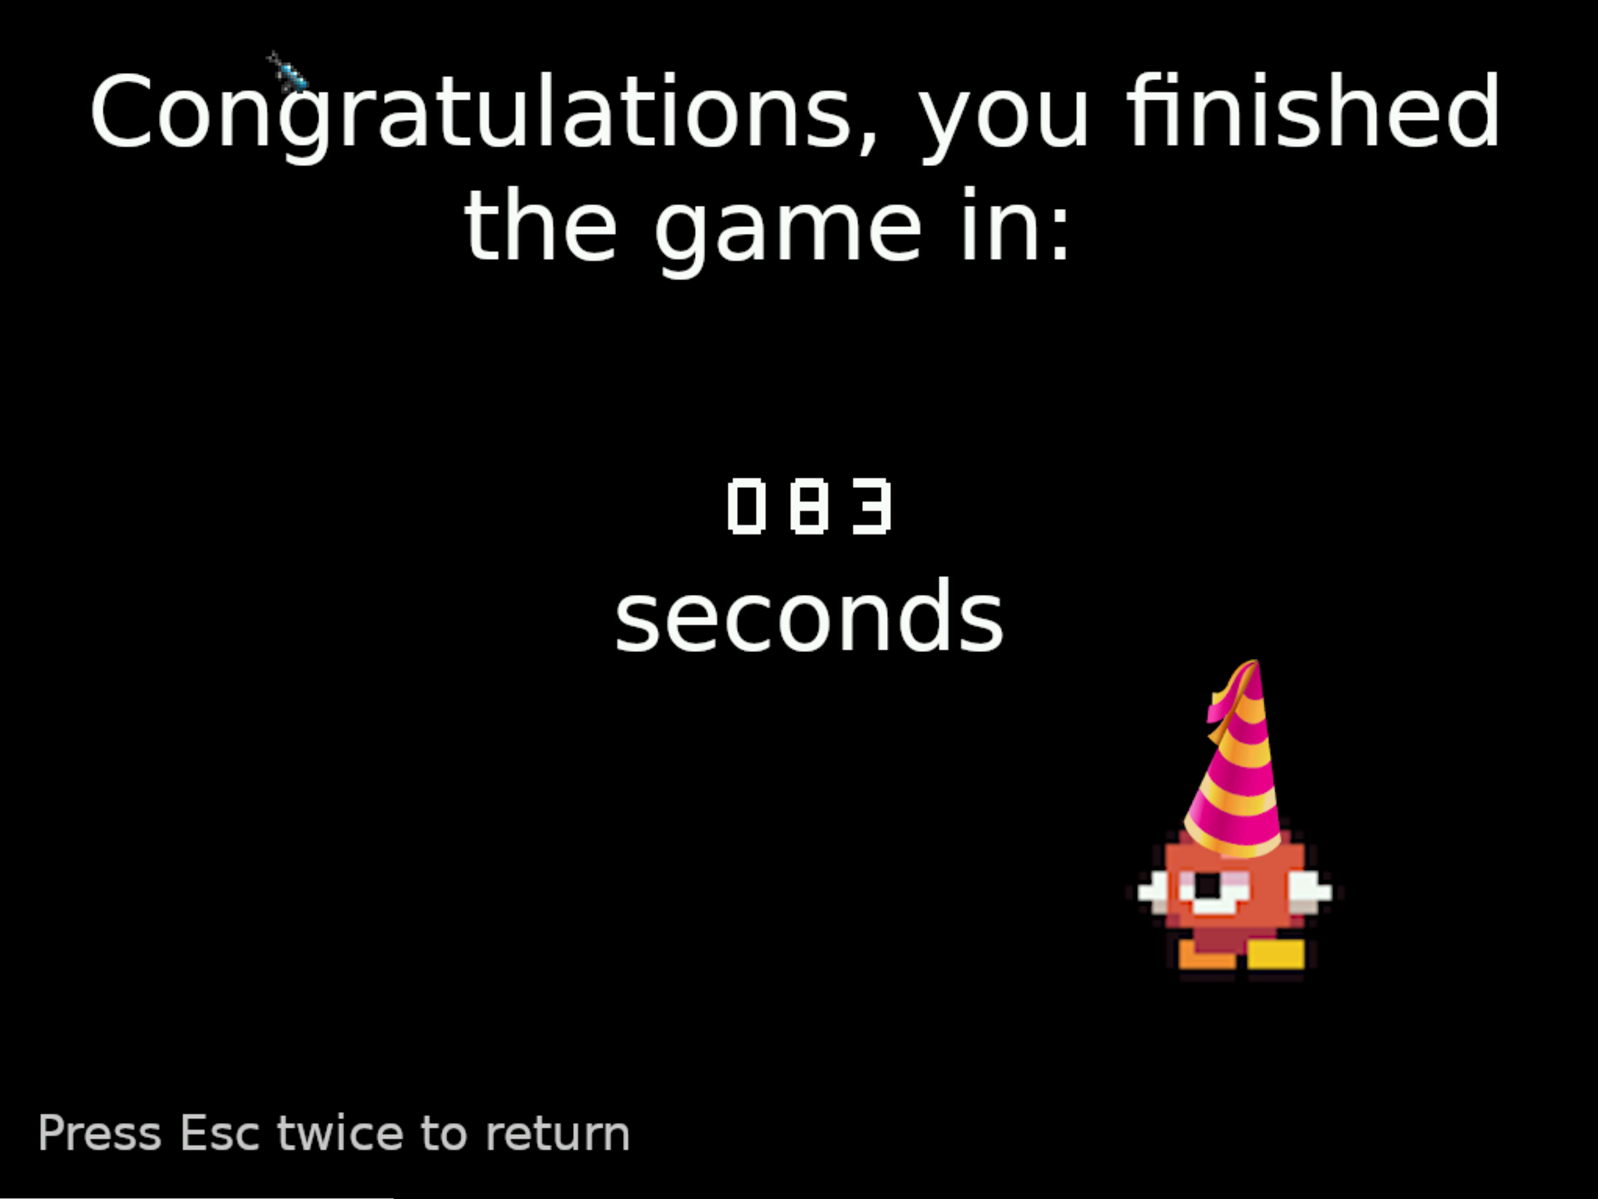
\includegraphics[width=0.8\textwidth]{win_screen}
	\caption{Campaign - Victory Screen}
\end{figure}

\pagebreak

\section{Arcade}

\textbf{\textit{Arcade}} é um modo de jogo alternativo, baseado na mecânica de \textbf{anti-gravidade} do outro modo de jogo. Neste o jogador terá de se desviar de \textbf{lasers} que vêm na sua direção (passando por entre estes) tentanto aguentar o máximo de tempo possível sem tocar neles e perder. Por cada par de \textbf{lasers} que o jogador passa o seu \textbf{\textit{score}} (\textbf{canto superior direito} - Figura \ref{fig:arcade_singleplayer}) aumenta por um ponto. O \textbf{\textit{score}} superior, a \textbf{branco}, representa a sua pontuação atual (que é reposta de cada vez que este toca num \textbf{laser}), já o \textbf{\textit{score}} inferior, a \textbf{cinzento}, representa a maior pontuação (\textbf{\textit{highscore}}) do jogador que ele conseguiu obter durante a partida.

Possui também um modo \textbf{\textit{versus}}, em que dois utilizadores jogam simultaneamente para ver quem obtém a maior pontuação. Para distinguir entre os dois jogadores, um deles é apresentado com uma cor \textbf{azulada}, tal como o seu \textbf{\textit{score}} (Figura \ref{fig:arcade_versus}).

\begin{figure}[H]
	\centering
	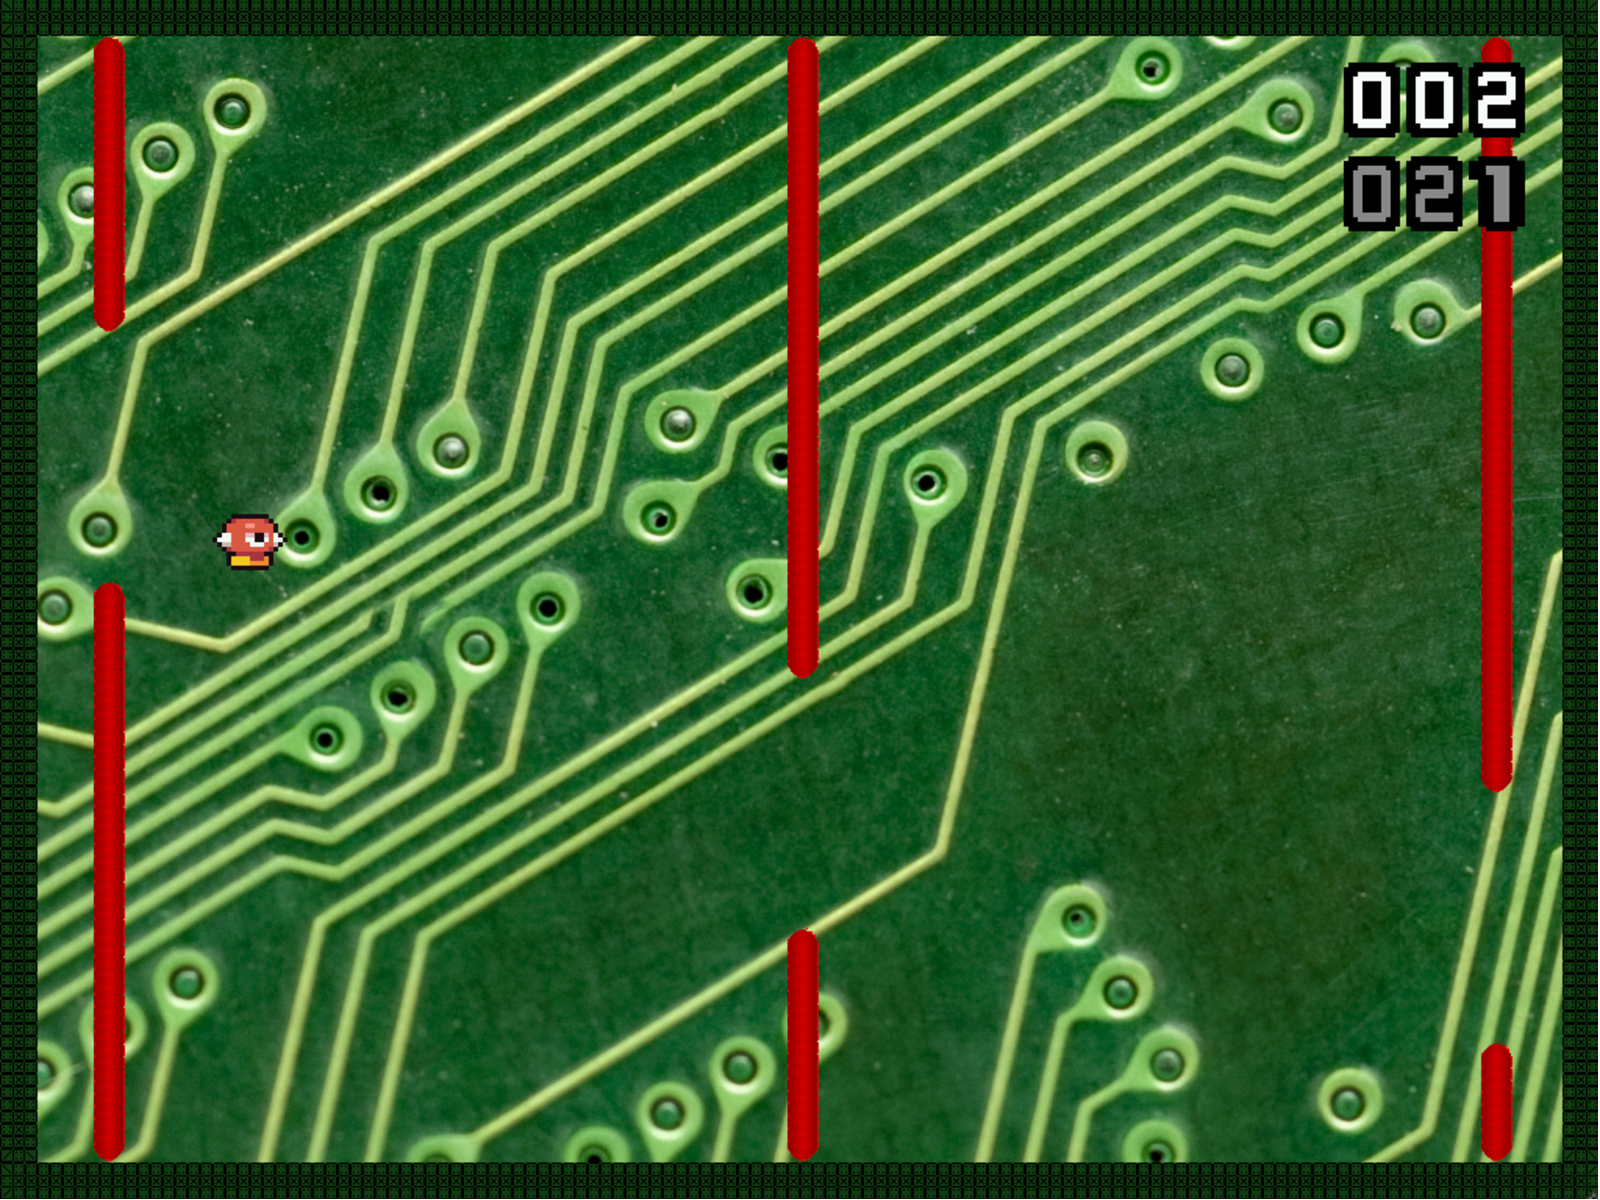
\includegraphics[width=0.6\textwidth]{arcade}
	\caption{Arcade - Singleplayer}
	\label{fig:arcade_singleplayer}
\end{figure}

\begin{figure}[H]
	\centering
	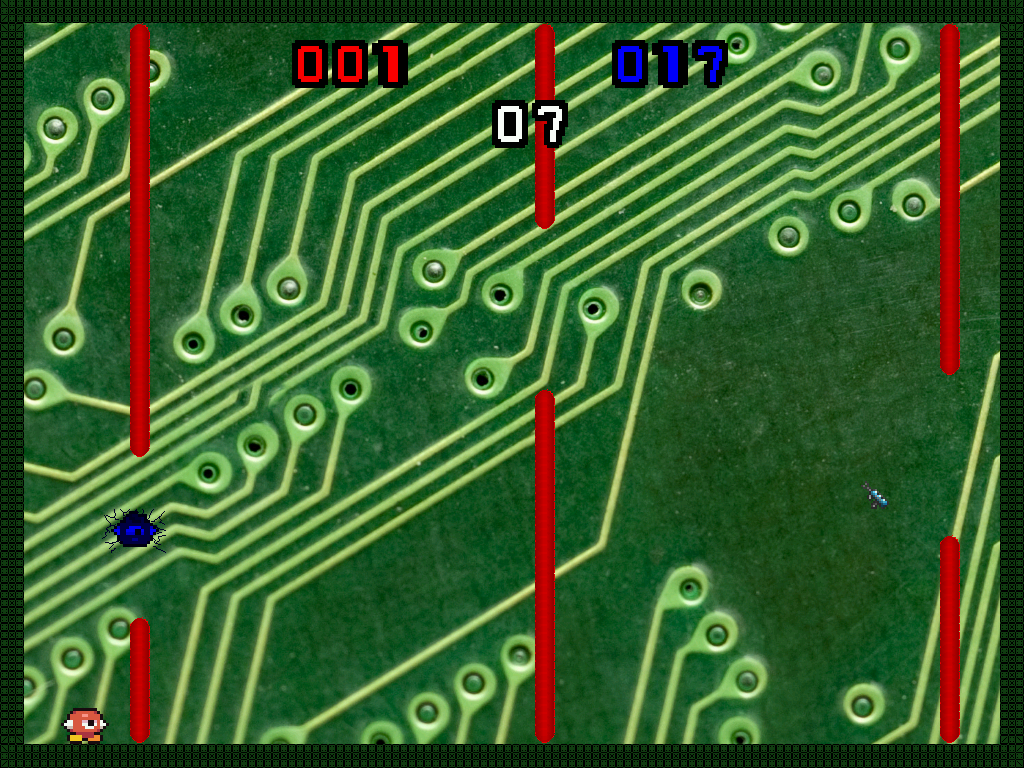
\includegraphics[width=0.6\textwidth]{arcade_versus}
	\caption{Arcade - Versus}
	\label{fig:arcade_versus}
\end{figure}

\chapter{Estado do Projeto}

\section{Dispositivos Usados}

\begin{center}
	\begin{tabular}{|c|c|c|} 
		\hline
			Dispositivo & Utilização & Interrupção \\ 
		\hline
		\hline
			Timer & Framerate handling  & Sim \\ 
			Teclado & Controlo da personagem 1 & Sim \\ 
			Rato & Menus e personagem 2 (switchboard) & Sim\\
			Placa Gráfica & Desenho dos menus e do jogo & Não\\
			Real Time Clock & Mini-game (switchboard) e tempo demorado (campaign) & Sim\\
			Serial Port & Modos Co-Op e Versus & Sim \\
		\hline
	\end{tabular}
\end{center}

\subsection{Timer}

O timer possui como principal função atualizar o estado do jogo, assim, a cada $\frac{1}{60}$s (o Timer 0 possui uma frequência de 60 Hz), todo a informação do nível (lasers ativos, coordenadas/estado do jogador, posição do rato...) é atualizada conforme os inputs do(s) utilizador(es) e é o mesmo é renderizado de acordo com essa informação.

\subsection{Teclado}

O teclado é usado para controlar a personagem 1 e o seu movimento, atraveś das teclas \textbf{W}, \textbf{A}, \textbf{S}, \textbf{D} ou pelas setas $\uparrow$, $\leftarrow$, $\downarrow$ e $\rightarrow$ e o seu salto pela tecla \textbf{Z} ou pelo \textbf{Espaço}.

Para além disso, se estiver a jogar em \textit{singleplayer}, o sentido da gravidade da personagem é trocado através da tecla \textbf{X}.

\subsection{Rato}

\paragraph{}
O rato é usado sobretudo no menu principal para selecionar o modo de jogo, clicando no botão correspondente, e no modo \textit{campaign} para controlar os \textit{sliders}, clicando e arrastando o botão esquerdo (o mesmo para a \textit{knob} no modo \textit{Co-Op}) e para selecionar o botão do \textit{laser} inativo.  

\subsection{Placa Gráfica}

\paragraph{}
A placa gráfica é usada para renderizar todo o jogo, por \textbf{camadas}(conforme a ordem das chamadas de render de cada elemento). É usada no modo \textbf{0x117}, que possui resolução \textbf{1024x768} e profundidade de cor \textbf{RGB 5:6:5} ($2^{16}$ cores possíveis).
Para além disso, usámos a técnica de \textbf{\textit{double buferring}} e a nossa taxa de atualização do ecrã é de \textbf{60 \textit{frames} por segundo}.

\subsection{Real Time Clock}

O \textbf{\textit{RTC}} é usado essencialmente em duas vertentes diferentes: No modo \textbf{\textit{Campaign}}, com a \textbf{personagem 1}, para ler a hora de quando a personagem inicia o jogo e de quando acaba para ver quanto tempo demorou a concluir o nível e com a \textbf{personagem 2} (\textit{switchboard}) para determinar de quanto em quanto tempo surgem os \textbf{\textit{balões}} do mini-jogo, através de \textbf{\textit{alarmes}} (\textit{interrupts}).

\subsection{Serial Port}

\paragraph{}
A \textbf{\textit{serial port}} é usada para coordenadar os dois jogadores conetados nos modos \textbf{multiplayer} (Campaign - Co-Op e Arcade - Versus). No \textbf{primeiro}, as personagens 1 e 2 são controladas pelos utilizadores em máquinas separadas, sendo que estas interegam entre si do seguinte modo: A personagem 2 envia a informação no que toca aos aspetos que esta pode alterar (altura do salto, velocidade...) à personagem 1 e esta envia informação acerca do estado do jogador (powerups obtidos, morto ou vivo...).

Já no modo \textbf{Arcade - Versus}, ambas as máquinas controlam a personagem 1 (Watt), aparecendo assim dois deles, um com a cor normal e um azul para distinguir entre os jogadores. Uma das máquinas age como \textbf{\textit{master}}, enquanto que a outra possui o papel de \textbf{\textit{slave}}. A \textbf{\textit{master}} fica encarregue de gerar a altura dos lasers aleatoriamente e envia essa informação para a \textbf{\textit{slave}}. Indiferentemente ao papel de cada máquina, tanto uma como a outra partilham informação da posição do jogador no ecrã, se está morto (para repor os lasers e posições dos jogadores) ou não e o seu score foi incrementado.

Implementada com FIFOs.

\chapter{Organização e Estrutura do Código}

\section{Geometry}

\paragraph{}
O módulo \textit{Geometry} é dividido em duas partes, \textit{Vec2d} e \textit{Rect}, e serve como base do nosso sistema de coordenadas, físicas, hitboxes e colisões. 
\subsection{Vec2d}

\paragraph{}
Este módulo é usado para representar vetores de duas dimensões, e consequentemente, pontos no espaço. Cada \textit{vec2d} é composto pelas suas componentes horizontal (x) e vertical (y), seguindo o referencial do frame buffer (x no sentido da esquerda para a direita e y no sentido de cima para baixo).

Existe um conjunto de operações que podemos efetuar com esta classe, nomeadamente somar, subtrair, multiplicar por um escalar, a norma do vetor, o ângulo entre dois vetores (usado para a \textit{Knob}), produto escalar, a distância entre dois pontos do plano, calcular a posição de um ponto em coordenadas polares, entre outros (todas estas funções encontram-se expostas no Doxygen deste módulo).

\subsection{Rect}

\paragraph{}
Este módulo é usado para colisões e para o UI. 

\subsection{Sistema de Colisões}

\paragraph{}
Sistema de colisões. \newline

Módulo desenvolvido por: 

\section{Bitmap}

\paragraph{}
O código que usamos ler bitmaps foi parcialmente retirado da internet, mas com várias alterações para melhor se ajustar ao tipo de \textbf{\textit{bitmaps}}que usamos (criados no GIMP).

Todos os ficheiros externos necessários (\textit{bitmaps}) encontram-se organizados dentro de uma pasta \textbf{\textit{assets}}, cuja localização pode ser específicada ao iniciar o jogo (até um limite de 255 caracteres, incluindo os ficheiros no interior dessa pasta).

Com o intuito de reduzir a quantidade de \textit{bitmaps} criados, ao desenhar no ecrã cada \textit{bitmap} normal, existe a opção de o desenhar alinhado à \textbf{esquerda}, ao \textbf{centro} ou à \textbf{direita} do ponto do ecrã indicado num argumento. Para além desse argumento existe ainda a possibilidade de desenhar o \textbf{simétrico} de cada \textit{bitmap} segundo quer o seu eixo (centrado no \textit{bitmap}) horizontal, vertical ou ambos. Esta segunda \textit{feature} foi especialmente útil e importante para as animações do jogador. 

Ao desenvolver o projeto considerámos necessário uma maneira de poder renderizar todas as nossas plataformas, paredes, espinhos e lasers de uma maneira mais dinâmica, para evitar criar uma nova sprite manualmente por cada objeto novo dessas classes. Assim implementamos uma função bitmap\_draw\_dynamic() que nos permite criar \textit{bitmaps} bastante reduzidos e que ocupam extremamente pouca memória RAM. Cada um destes \textit{bitmaps} pode ser subdividido em 9 quadrados, todos de tamanho igual, específico de cada imagem. A função irá depois reproduzir cada secção apropriadamente para produzir no ecrã uma imagem do tamanho pretendido.

Existe ainda a possibilidade de cada pixel ser "multiplicado" por uma cor. Devido ao custo pesado de computação desta operação, decidimos que usar uma operação bitwise entre a cor do pixel e da cor a multiplicar, visto que o efeito que ela produz seja satisfatório o suficiente para as nossas necessidades, mantendo um baixo custo computacional. Esta operação irá sempre escurecer a cor do \textit{bitmap} original, e quando aplicado a um pixel branco irá ficar apenas a cor a multiplicar. Esta propriedade foi usada a renderizar todas as plataformas e paredes. 

Todos os \textit{bitmaps} podem ser desenhados com "transparência", isto é, definimos a cor rosa, \textbf{0xFF00FF} (em RBG 888), como a cor que será sempre ignorada ao desenhar. \newline

Módulo desenvolvido por: Eduardo Correia (40\%) e Tiago Silva (60\%)
 
\section{Sprite}

\paragraph{}
No nosso programa existem duas classes de \textit{sprite}: a \textbf{normal} e a \textbf{dinâmica}. A dinâmica é usada sempre que quisermos usar a função bitmap\_draw\_dynamic() referida acima, a normal é usada em todos os outros casos.

Foi tomada a decisão de implementar as animações seguindo o popular \textit{Unity}. Este \textit{game engine} tem uma propriedade \textit{Animator} que pode ser acoplado a qualquer objeto com um \textit{Renderer}. O \textit{Animator} é apenas uma máquina de estados que indica, no momento de renderizar o objeto no ecrã, qual a \textit{Sprite}, textura ou \textit{3D Model} a usar.

O sistema que decidimos implementar está imbutido diretamente na nossa classe \textit{Sprite}, que permite criar cada objeto com até 255 \textit{bitmaps}. Para permitir a instanciação de tantos \textit{bitmaps}, recorremos a um construtor que aceita um número variável de argumentos. A nossa classe tem uma propriedade "estado da animação", que indica qual dos n \textit{bitmaps} a desenhar. Este estado pode obtido e alterado através de um par de setters e getters.

A máquina de estados responsável por controlar qual o valor deste estado (por \textit{default} este valor é 0, ou seja, o primeiro \textit{bitmap}). Este tema será abordado novamente ao discutir o \textit{player}.

Cada \textit{sprite} criada também tem um \textit{offset} individual que é utilizado ao renderizar o \textit{bitmap} no ecrã. Existe ainda um getter das \textit{sprites} (\textbf{Vec2d\_t sprite\_get\_size(Sprite\_t *s)})que permite obter o tamanho do primeiro \textit{bitmap} carregado, especialmente útil para obter dinâmicamente a \textit{hitbox} do \textit{player} e dos botões.\newline

Módulo desenvolvido por: Tiago Silva

\section{Game Manager}

Módulo desenvolvido por: 

\section{Hardware Manager}

\paragraph{}
Este módulo foi uma tentativa de tentar encapsular ao máximo todo o conhecimento e funções responáveis por interagir com o hardware num único sítio o e transparecer o mínimo possível sobre as nossas implementações internas do \textit{timer}, \textit{keyboard}, \textit{mouse}, etc..

Infelizmente existem outros módulos com um grande conhecimento destes protocolos, como o \textit{InputEvents}, o \textit{GameManager} e tudo o que envolvesse o \textit{serial port}.\newline

Módulo desenvolvido por: 

\section{Level}

Esta classe representa todo um nível e os seus constituintes (jogador, elementos UI, plataformas, lasers, espinhos...)
Vão haver essencialmente dois níveis, um para a Campaign --- new\_prototype\_level() e outro para Arcade\newline

Módulo desenvolvido por: Eduardo Correia (50\%) e Tiago Silva (50\%) 

\section{Switchboard}

\section{Player}

O módulo \textit{Player} trata de gerir a representação de um jogador e da sua interface no nosso projeto bem como a sua interação com os restantes módulos. 

\subsection{Player}

\subsection{PlayerTwo}

\paragraph{}
Apenas é utilizado no modo Arcade - Versus para representar um segundo jogador que está a jogar noutra máquina. 

Módulo desenvolvido por: Eduardo Correia (30\%) e Tiago Silva (70\%) 

\section{UI Elements}

O módulo \textit{UI Elements} possui diversas subdivisões, uma vez que utilizámos vários elementos bastante diferentes entre si de interface com o utilizador, sendo estes os seguintes.\footnotemark

\subsection{Button}

Tal como o nome indica, esta "classe" representa um simples botão com uma aparência desejada e formato retangular que pode ser clicado para ativar alguma funcionalidade.
Caso esteja ativo e o utilizador clicar nele com o cursor do rato, ativa a sua funcionalidade.

\subsection{Slider}

Uma barra vertical ou horizontal com um manípulo no seu interior que pode ser deslizado e colocado numa posição que provocará um efeito de \textit{magnitude} proporcional à posição do manípulo no \textit{Slider} relativamente à sua extremidade.

\subsection{Knob}

Uma espécie de "maçaneta" que pode ser rodada, clicando na sua extremidade com o botão esquerdo do rato e arrastando-a, ativando algum efeito durante o tempo que ocorre entre o instante em que é rodada até rodar de volta à sua posição inicial.

\footnotetext{Os três primeiros elementos possuem um estado de ativo ou inativo e a qualquer momento é possível mudar o seu estado --- set\_activation(). Caso um elemento esteja inativo, a sua cor aparece ligeiramente menos saturada e não é possível interagir com o mesmo, ou seja, se for um \textit{Button}, não é clicável, se for um \textit{Slider}, não é "deslizável" e por último, se for uma \textit{Knob}, não é "rodável". Se estiver ativo, a sua aparência é normal e já é interagível.}

\subsection{Number}

A "classe" \textbf{\textit{Number}} serve para representar um único algarismo entre 0 e 9, sendo ainda possível incrementá-lo dinamicamente por um unidade\footnotemark --- \textit{updade\_number()}.

\footnotetext{Caso o algarismo seja 9, passa para 0}

\subsection{Score}
\paragraph{}
A "classe" \textbf{\textit{Score}} serve para representar um número com um determinado número de algarismos (\textit{Numbers}). Possui como principal propósito apresentar a pontuação atual de um jogador no modo de jogo \textit{arcade}, porém, também é usada para exibir o tempo (em segundos) que o jogador demorou a concluir o nível do modo \textit{campaign}.

É possível iniciar o \textit{Score} com um valor inteiro positivo qualquer --- new\_score(), bem como repô-lo (colocar a 0) --- \textit{reset\_score()} ou mudar o seu valor --- \textit{set\_score()}. \newline

Módulo desenvolvido por: Eduardo Correia (30\%) e Tiago Silva (70\%) 

\section{Powerup}

\section{Timer}

\paragraph{}
\textit{Código importado do Lab 2}\footnotemark\newline

Módulo desenvolvido por: Eduardo Correia (50\%) e Tiago Silva (50\%)

\section{Keyboard}

\paragraph{}
Para guardar o input do \textit{keyboard} recorremos à classe \textit{KbdInputEvents}, que mantém um registo sobre todos os \textit{scancodes} de 1 \textit{byte} e sobre um subset específico de \textit{scandodes} de 2 \textit{bytes}.

Com o propósito de criar um \textit{dispatcher} eficiente, foi usado um \textit{map} para mapear cada \textit{scancode} ao seu valor respetivo. É registada sempre se uma tecla está a ser pressionada e se uma tecla foi pressionada durante este frame (isto é, se o utilizador empurrou para baixo a tecla).

A função \textbf{kbd\_input\_events\_process\_scancode()} trata de interpretar qualquer scancode que seja recebido do \textit{keyboard}.

Para mais permito um acesso mais simples a estas informações a partir de qualquer ponto do programa, esta classe foi tornada um \textit{singleton}, com dois getters para saber se uma tecla se encontra premida, \textbf{get\_key(KeyboardMap\_t map)}, e se uma tecla foi premida neste frame, \textbf{get\_key\_down(KeyboardMap\_t map)}.

O \textit{KeyboardMap} utilizado como argumento é um \textit{enum} com todas as teclas suportadas. Isto também permite que se o layout do teclado for diferente do \textit{default}, os scancodes podem ser alterados apenas nesse \textit{enum}.

Para detetar se uma tecla foi premida num certo frame, foi necessário limpar esse segundo map no final de cada frame, isto é, após a chamada da função \textit{update()}, para garantir que os inputs são interpretados corretamente, recorrendo à função \textbf{reset\_kbd\_input\_state()}.\newline

\textit{Código importado do Lab 3}\footnotemark[\value{footnote}]\newline

Módulo desenvolvido por: 

\section{Mouse}

\paragraph{}
Para abordar completamente o uso mais direto do \textit{Mouse} é necessário cobrir duas partes, o \textit{MouseInputEvents} e o \textit{MouseCursor}, sendo que o segundo tira partido do primeiro.
Tal como o \textit{KbdInputEvents}, estas duas classes são também \textit{singletons}.

\subsection{MouseInputEvents}

\paragraph{}
Esta "classe" guarda e expõe para o resto do programa os botões premidos pelo utilizador, se eles estão a ser premidos neste instante e se eles começaram a ser pressionados neste frame. Regista também o \textit{delta} do movimento do rato no eixo do x e y em cada frame.

Para permitir saber se um dado botão começou a ser premido num determinado frame e para garantir que o \textit{delta} do rato entre frames é o correto, recorremos ao mesmo truque do \textit{KbdInputEvents}, utilizando a função \textbf{reset\_mouse\_input\_state()}.

\subsection{MouseCursor}

\paragraph{}
Representa o cursor do rato\newline

Módulo desenvolvido por: 

\section{Video}

\textit{Código importado do Lab 5}\footnotemark[\value{footnote}]

\footnotetext{No código importado dos labs fizemos ligeiras alterações, como remover funções que não utilizamos (por exemplo, naquilo em que optássemos por usar \textit{interrupts} removemos o código que lidava com \textit{pollling}) e especificar uma abordagem geral para uma específica ao projeto, para ser mais eficaz (como usar a placa gráfica num modo apenas, correspondente ao que optámos por utilizar no nosso jogo).}

\section{RTC}

O módulo do RTC é responsável por obter informação acerca da hora atual --- \textit{get\_date()} possuindo uma verificação antes de o fazer para obter a hora correta, bem como programar alarmes. --- \textit{rtc\_set\_alarm()}. --- rtc.c \newline

Módulo desenvolvido por: Eduardo Correia

\section{UART}

Módulo desenvolvido por: Eduardo Correia (20\%) e Tiago Silva (80\%)
 
\section{Proj}

%O módulo \textit{Proj}, por mais que possa parecer contra-intuitivo, é dos que menos tem peso no projeto, uma vez que só trata de chamar a função de iniciar o jogo --- \textit{start_game}. O \textit{GameManager} trata de tudo o resto.

\section{Call Graph}

TODO: Adicionar o call graph de cada updade e render sozinhos e explicar

\section{Peso Relativo dos Módulos no Projeto}

\begin{center}
	\begin{tabular}{|c|c|} 
		\hline
			Módulo & Peso relativo \\ 
		\hline
		\hline
			Geometry & \\
			Bitmap & \\
			Sprite & \\
			Game Manager & \\
			Hardware Manager & \\
			Level & \\
			Switchboard & \\ 
			Player & \\
			UI Elements & \\
			Powerup & \\
			Timer & \\
			Keyboard & \\
			Mouse & \\
			Video & \\
			RTC & \\
			Proj & \\
		\hline
	\end{tabular}
\end{center}

\chapter{Detalhes de Implementação}

% É possível mudar o path absoluto das imagens com um argumento da linha de comandos.

\chapter{Conclusões}

\paragraph{}

\end{document}